\section{Data Description}

\subsection{Prices, Exchanges, and Coin characteristics}


\begin{figure}[h]
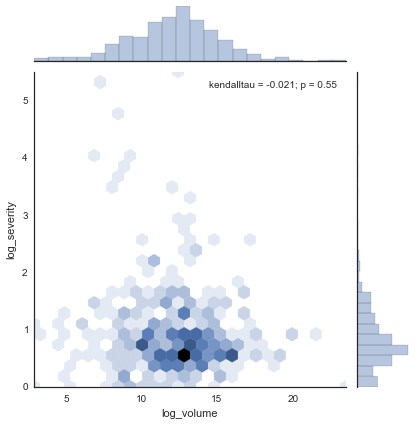
\includegraphics[width=\columnwidth]{severity_volume}
\end{figure}

Our main outcome measures are the severity of drop in the value of a unit of the asset, and the magnitude in USD of the transactions in it.
We scrape daily price and volume data from coinmarketcap.com\footnote{ For robustness analysis smaller subsets of the coins where available from coin }
%JULIAN: Didn't follow the above footnote
We operationalize the severity of a bubble as the inverse of 1 dollar that would be lost buying at the maximum price and selling after that proportionally to the volume of the market until the present; we call this severity.
%JUliAN: Above is hard to follow if not spelled out in the form of equations; wordy papers with everything explained inline seems more economics and less WWW
We define the volume as the sum of the dollar volume of trade reported over all exchanges.
